%
% Chapter 4
%

\chapter{multiPANTS}

% Collab note
% PANTS collab
% RNAseq gen and quant
% Cell count estimates

\begin{outline}

\section{Introduction}

\subsection{IBD}

\1 IBD is a complex IMID of the GI tract.
    \2 Prevelance of IBD in the Western world is at least 0.5\%, and rising \url{https://www.nature.com/articles/nrgastro.2015.150}.
    \2 Although often seen as a disease of the Western world, the disease is increasingly common in non-Western countries as they industrialise.
    \2 Pathogenesis defined by interaction of the host genetic, environmental (e.g. diet) and gut microbial factors \url{https://www.nature.com/articles/nrgastro.2015.186}

\1 It has two major forms, UC and CD.
    \1 UC is distinguished by ...
    \2 CD is distinguished by ... \autocite{roda2020CrohnDisease}

\1 IBD is one of the most-well studied diseases by GWAS
    \2 Over TODO hits at TODO loci (dig up latest paper out of \autocite{delange2017GenomewideAssociationStudy,huang2017FinemappingInflammatoryBowel,luo2017ExploringGeneticArchitecture})
    \2 Genetic correlation between UC and CD is high
    \2 Hits unique to CD are TODO

\subsection{Anti-TNF therapies for IBD}

\1 anti-tnfs in use for IBD
    \2 also used in related conditions e.g. RA \autocite{mulhearn2019UsingImmunophenotypePredict}
    \2 "Biologic therapy with anti-TNF agents." for IBD \url{https://www.nature.com/articles/nrgastro.2015.135}
        \3 Two big players: adalimumab and infliximab \autocite{adegbola2018AntiTNFTherapyCrohn}
        \3 \url{https://www.nice.org.uk/guidance/ta329}
        \3 promote mucosal healing
        \3 Their mechanisms of action on the target pathway \autocite{levin2016MechanismActionAntiTNF}

\1 failure of anti-tnfs is common (TODO\%) \url{https://journals.lww.com/ctg/Fulltext/2016/01000/Loss_of_Response_to_Anti_TNFs__Definition,.2.aspx}
    % "[3] FlamantM, Roblin X. Inflammatory bowel disease: towards a personalizedmedicine.  Ther Adv Gastroenterol 2018;11:1756283X17745029."
    % For anti-TNF therapy in particular, primary nonresponse
    % rates vary from 10 to 30%, and the annual risk of secondary
    % loss of response ranges from 13% for infliximab (IFX) to 20% for
    % adalimumab (ADM) [3].
    % 4 Ben-Horin S, Kopylov U, Chowers Y. Optimizing anti-TNF treatments in inflammatory bowel disease. Autoimmun Rev 2014;13:24–30.
    % This practice is associated with insufficient remission rates
    % that results from primary non-response (20%–40% in clinical
    % trials; 10%–20% in real-life cohorts)4
    \2 types of failure: \gls{PNR}, non-remission, adverse events.
        \3 clinical predictors \autocite{kennedy2019PredictorsAntiTNFTreatment}
        \3 immunogenicity (not a failure, but mediates it) via anti-drug Abs
        % Furthermore 10-40% of patients fail to respond to 10-12 weeks of therapy (primary non-response - PNR), and a further 23-46% lose response (loss of response – LOR) after 12 months of treatment.

\1 although reported failure rates (single-measure) do not necessarily reflect that there is something inherent to an individual that causes it \url{https://www.ncbi.nlm.nih.gov/pmc/articles/PMC524113/} senn2016MasteringVariationVariance
    % Genome-wide association studies (GWAS) have proven to be a more successful approach for this objective. To date, eight GWAS on anti-TNF response in RA have been performed (22–29), identifying several loci associated at a genome-wide scale. From these, variation at MED15, GFRA1, PDE3A-SLCO1C1, and CD84 has been replicated in, at least, an independent cohort of patients (30).
    \2 GWAS studies in RA \url{https://www.ncbi.nlm.nih.gov/pmc/articles/PMC6614444/}
    % Several attempts have been made to define a baseline signature
    % of anti-TNF response in patients with IBD using genetics,7 8
    % microbiome9 and gene expression data.10–13 Yet, no predictive
    % biomarker is in clinical practice.
    \2 attempts in IBD \autocite{gaujoux2019CellcentredMetaanalysisReveals}
    \2 furthermore we know immunogenicity has genetic determinant \autocite{sazonovs2019HLADQA105Carriage}
    \2 does not necessarily share the same genetic arch as disease risk
    \2 if heritable, and amenable to gwas, follow the same strat of gene prioritisation for failure phenotypes, to drug target prioritisation as outlined in ch1
    \todo{make sure some statement of drug target prioritisation is in ch1}

\1 Biologics are part of a whole treatment pyramid \url{https://www.nature.com/articles/nrgastro.2013.158}
    \2 biologics are the 2nd most intense therapies below surgical intervention
    \2 Step-up approach: undertreats patients
    \2 Step-down approach: exposes patients to risks from more aggressive therapies
    \2 Neither are ideal

\1 The promise of transcriptomic signatures for response prediction and stratifying patients to the right therapies
    \2 much like for sysvacc in ch2
    \2 starts with DGE R vs NR in biopsies
    % verstockt2019LowTREM1Expression
    % Gene expression analysis of inflamed biopsies
    % of Crohn's disease (CD) and ulcerative colitis patients (UC) prior
    % to IFX therapy, identified several genes differentially expressed
    % between responders and non-responders [6–8].
    % Finally,
    % advanced bioinformatic techniques integrated all publically available
    % datasets and identified colonic expression of both oncostatin
    % M (OSM) and Triggering Receptor Expressed on Myeloid cells 1
    % (TREM1) as key players in and predictors of anti-TNF (non-)responsiveness
    % [11–13].
    \2 cause or effect?
    \2 conflict in existing studies e.g. \enquote{The difference in results of these two studies could not be more stark: one found that TREM1 was downregulated in anti-TNF responders, and the other found that TREM1 was downregulated in anti-TNF non-responders.} \url{https://www.nature.com/articles/s41575-019-0228-5}
        % \3 <Also grep other signatures from this paper>
    \2 TREM1 signature \autocite{verstockt2019LowTREM1Expression}
        \2 prospective study of 54 active IBD patients (24CD, 30UC)
        % at baseline
        % validated whole blood TREM1 as the first predictive signal for
        % anti-TNF induced endoscopic remission in a mixed cohort of patients
        % with both Crohn's disease or ulcerative colitis.
        % anti-TNF specific
        % In the anti-TNF cohort, TREM1 was significantly downregulated at
        % baseline in patients achieving endoscopic remission (fold change (FC)
        % = 0.67, p b .001) (Fig. 1A).
        % Logistic regression analysis identified total whole blood TREM1 mRNA expression as the only significant predictor of anti-TNF induced endoscopic remission (p = .02). ROC analysis based on baseline TREM1 mRNA levels in the anti-TNF cohort, gave an area under the curve (AUC) of 77.7% (95% CI 65.2–90.1%, p = .001).
        % TREM1 is a receptor expressed on innate immune cells, known to
        % amplify inflammatory signals that are initially triggered by Toll-like receptors
        % and thus contributing to the pathophysiology of many acute and
        % chronic inflammatory conditions [19].

\subsection{The PANTS cohort}

% NOTE: here is overall structure of existing study
% 1241 patients were assessable at week 14. Primary nonresponse
% occurred in 170 (21·9%, 95% CI 19·1–25·0) of
% 775 patients treated with infliximab and 125 (26·8%,
% 22·9–31·1) of 466 patients treated with adalimumab
% (table 2). After excluding primary non-responders,
% the estimated proportion of infliximab-treated patients
% who had loss of response by week 54 was 36·9%
% (32·7–40·9), and for adalimumab was 34·1% (28·4–39·4;
% appendix pp 15–16). At week 54, 469 (60·9%; 57·4–64·0)
% of 770 infliximab-treated patients were classified as
% being in non-remission, compared with 295 (66·9%;
% 62·3–71·3) of 441 adalimumab-treated patients (table 2).
\1 prospective, observational cohort study UK wide, with total enrolled n=1610 , 92.29pc EUR \autocite{kennedy2019PredictorsAntiTNFTreatment}
% \1 "To measure the clinical, biological, genetic markers that define response to anti-TNF in patients with active Crohns disease [ Time Frame: 3 years ]"
    \2 patients at least 6yo, with active luminal CD, and antitnf naive
        \3 active defined by CRP and faecal calprotectin
    \2 up to 12 mo of followup (until withdrawl due to remission or otherwise), possible 2y extension
    \2 2 drugs: ada and inf
    \2 evaluates several aspects of antitnf response: PNR at week 14, non-remission at w54, adverse events
        \3 also immunogenicity (defined by antidrug ab levels)
    \2 PNR evaluated at w14 via algo, after PNR (24\%), rarely helpful to keep dosing
    \2 immunogenicity (63pc adalimumab), (28.5pc infliximab)
        \3 use of immunomods had protective effect on time to immunogenicity 
    \2 8\% have an adverse drug reaction that curtails treatment
    \2 clinical factors associated with response
        \3 low serum drug concentration in peripheral blood at w14 (ELISA) assoc with PNR and non-remission and immunogenicity, (in multivariate models, for both drugs) 
        \3 optimal is conc above which there is no improvement
    \2 suggest Dose intensification

% The HLA-DQA1*05 allele, carried by approximately 40% of Europeans,
% significantly increased the rate of immunogenicity (hazard ratio [HR],
% 1.90; 95% confidence interval [CI], 1.60–2.25; P ¼ 5.88  10–13).
% Both drugs, and regardless of immunomodulator
% Dominant effect
\1 in this cohort, immunogenicity has a genetic association \autocite{sazonovs2019HLADQA105Carriage} 

\subsection{chapter summary}

\1 What is the hypothesis???
\1 Identifying signatures of PNR
    \2 replicate TREM1?
\1 Identifying reQTL
    \2 Why require a reQTL approach?
    \2 There are IBD specific reQTL (TODO is that relevant?) \autocite{piasecka2018DistinctiveRolesAge}
    \2 identify reQTL for use in e.g. mediation analysis of the genetic causes of non-response via expression

\section{Methods}

\subsection{Overall strategy}

% https://discourse.datamethods.org/t/responder-analysis-loser-x-4/1262
% Responder analysis is a 4-fold loser. It fails to give the needed clinical
% interpretation, has poor statistical properties, increases the cost of studies
% because binary outcomes require significantly higher sample sizes, and raises
% ethical issues because more patients are required to be randomized than would
% be needed were the endpoint and analysis to be fully efficient.

\subsection{Study design}

% Visit info from protocol
%
% visit_1
%     This visit must occur in the 7 days prior to commencing anti-TNF medication, and preferably on the day of the first infusion / injection
% visit_1X
%     3 days after first dose of anti-TNF therapy - OPTIONAL
% visit 2 (not in phenotypes)
%     w12
%     The patient’s gastroenterologist will decide whether to continue with the next infusion / injection at week 14, or stop, anti-TNF therapy.
%     NB if after this visit, the anti-TNF drug is stopped, or switched to an alternative anti-TNF drug then the patient’s next visits will be Exit visit 1 (scheduled for week 14) and Exit visit 2 (scheduled for week 22, patients on IFX, week 28 patients on ADA)
% visit_3
%     w14
%     Immediately prior to IFX infusion, ADA injection
% exit_1
%     Exit Visit 1 (Withdrawal of anti-TNF therapy before week 54 or non-elective withdrawal after week 54).
    % If the drug is withdrawn, or the patient switched to another anti-TNF drug, two study exit visits will be scheduled. Exit visit 1 is scheduled for 8 weeks after the last IFX infusion or 2 weeks after the last ADA injection. Exit visit 2 is scheduled for 16 weeks after the last IFX infusion or ADA injection.
% lor_3
%     Loss of response (LOR) will be defined after week 13 by reviewing the following:
%         Initial response to anti-TNF defined at week 12.
%         Symptomatic inflammatory IBD activity, which is of sufficient severity and duration to warrant an escalation in steroid, immunomodulatory, or anti-TNF therapy or surgical resection as directed by the patient’s gastroenterologist.
%         Patients who lose response before week 13 will be categorised as primary non-responders
%     The LOR visit should be scheduled immediately prior (preferably on the same day) to the next (modified) anti-TNF infusion / injection and will replace any standard visits. In the event of anti-TNF dose intensification this visit may occur earlier than planned or may involve a higher dose of anti-TNF drug.
%     NOTE: this means visits still continue to be scheduled as long as
%         For IFX:
%             Conduct LOR 1 visit which will replace the standard visit.
%             Standard visits will continue to be scheduled for each subsequent IFX infusion up to week 54.
%         For ADA:
%             Conduct LOR 1 visit which may replace a standard visit if this coincides with the scheduled ADA research visits at week 30 and week 54
%             After the LOR1 visit subsequent visits are scheduled every 3 months for 12 months. These visits may coincide with the scheduled research visits 4, 5, 6, 7, 8 and 9. If this is the case simply use these visits and labels. If not then use LOR 2 or LOR ES visits and labels.
% lor_4
% visit_4
%     w30
%     Immediately prior to IFX infusion, ADA injection
% visit_5
%     w54
%     Immediately prior to IFX infusion, ADA injection
%
% AbbVie definition of w14 timepoint:
%
% Excluding visits labeled “visit_1X” (72 hour visit), we labeled the first follow-up visit after baseline as a “primary_response” visit if it occurred <= 20 weeks after baseline, in line with what was reported in the paper, and independent of whether it was labeled “visit_3” or “exit_1” or “lor_3”.
%
Patients recruited to the \gls{PANTS} study may attend up to 10 study visits, a detailed overview of which can be found in \textcite{kennedy2019PredictorsAntiTNFTreatment}. 
This chapter focuses on the four major study visits: week 0 (week \numrange{-4}{0}), week 14 (week \numrange{10}{20}), week 30 (week \numrange{22}{38}), and week 54 (week \numrange{42}{66}).
Time is measured relative to the day of the first drug dose.
Ranges indicate the eligibility windows defined in \textcite{kennedy2019PredictorsAntiTNFTreatment}.
Major visits were scheduled prior to drug doses (IFX infusion or ADA injection).
At each major visit, peripheral whole blood samples were collected and preserved in Tempus™ Blood RNA Tubes
\todo{figure out how many doses happen at additional visits}
For this chapter, samples from scheduled major visits that fall outside the windows were included.
Samples from additional visits (e.g. scheduled due to \gls{LOR} or early study exit) that fall into major visit windows were also included, as additional visits often replaced major visits for patients with \gls{PNR} or \gls{LOR}.
% TODO: add figure ref

\begin{figure}
    \centering
    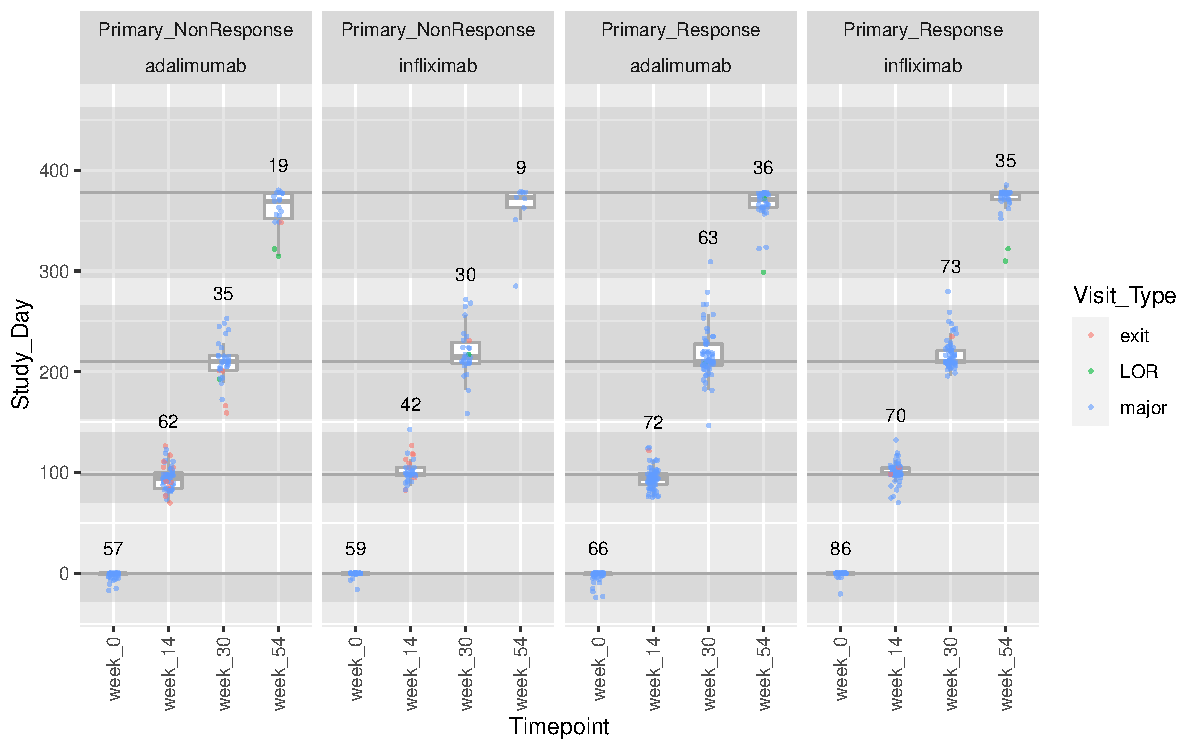
\includegraphics[width=1.0\textwidth,page=1]{mainmatter/figures/chapter_04/process_pheno.pheno_filtered_dge.Study_Day_vs_Visit_Label.pdf}
    \caption{}
    \label{fig:multipants_studyDay_boxplots}
\end{figure}

\begin{figure}
    \centering
    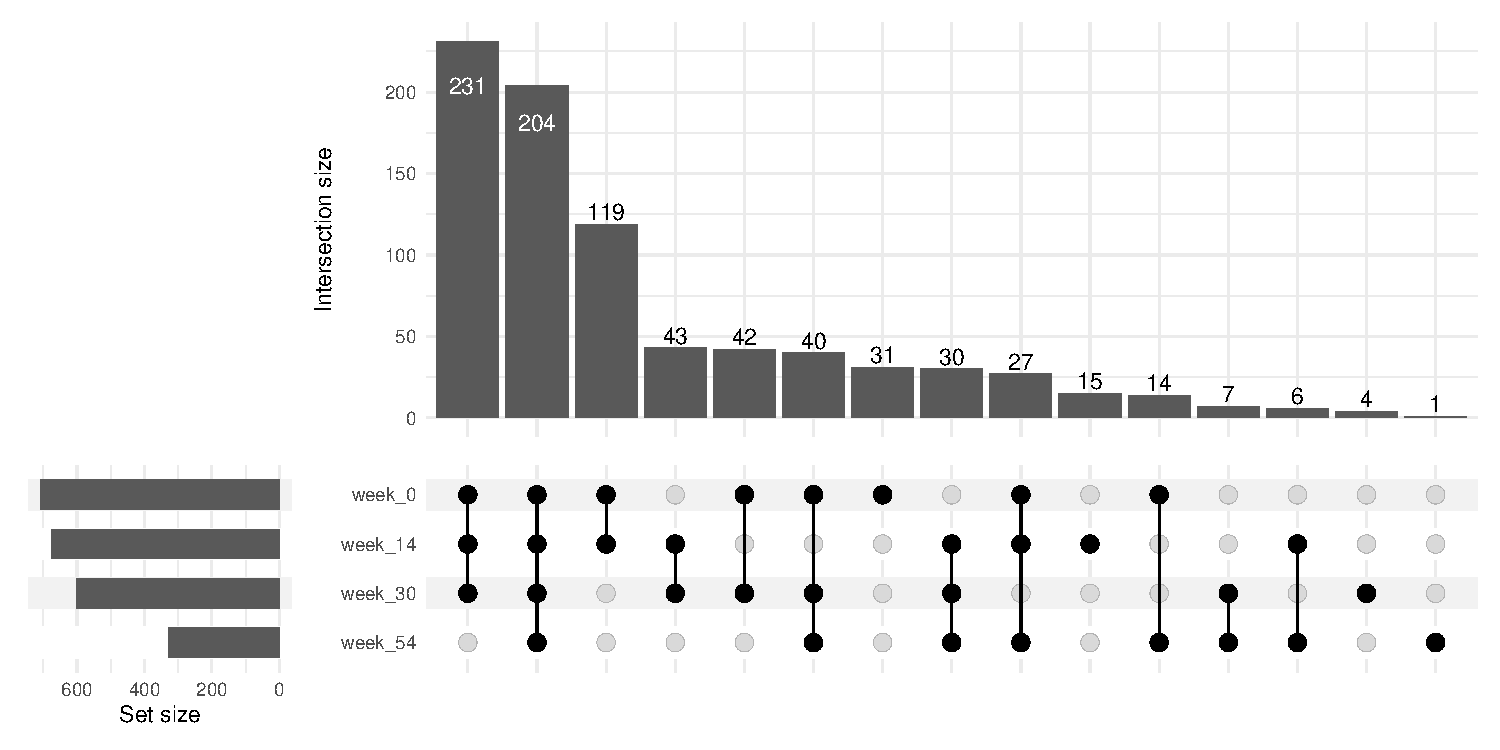
\includegraphics[width=1.0\textwidth,page=1]{mainmatter/figures/chapter_04/process_pheno.pheno_filtered_dge.Visit_Label_upset.pdf}
    \caption{}
    \label{fig:multipants_visits_upset}
\end{figure}

\subsection{Definition of \glsfmtfull{PNR}}

% Selection criteria for samples from Nick:
%
% ~200 for each drug, ~100 PNR, 100 remission. PNR had to be PNR at week 14 and non-remission at week 54 (or unknown at week 54). Remission had to have active disease at baseline and be in remission or response at week 14 and remission at week 54 (or unknown at week 54 and remission at week 30).
% ideal_downstream_cohort <- bd_vr_clin %>%
%   filter(
%     (crp_visit_1 >= 4 | calpro_visit_1 > 100),
%     (pnr & (is.na(remission_visit_5) | !remission_visit_5)) |
%     ((status_visit_2_3 %in% c("Response", "Remission")) & (remission_visit_5 | (is.na(remission_visit_5) & remission_visit_4)))
%   )
% They also had to be 16 years or over and have a baseline serum sample. Within the infliximab patients, there was propensity matching between PNR/non-PNR based on on_imms_visit_1 + on_steroids_visit_1 + age_at_first_dose + earliest_weight_category_4 + albumin_visit_1 + sex.
\1 \gls{PNR} was defined as <...>
\1 "In the event of loss of response (LOR) an additional LOR visit will be scheduled to occur immediately prior to the next anti-TNF infusion / injection.  Patients will remain in the study if they continue with the same anti-TNF drug, even if LOR or ADRs occur."

\subsection{RNAseq data generation and quantification}

% From Mark:
% Here is an extended version of the protocol, with highlighting of the portion on poly-A selection and subsequent depletion steps:
%
% RNA and DNA were isolated from whole blood samples collected in Tempus Blood RNA Tubes.
%
% The Applied Biosystems Tempus Blood RNA Tube and Tempus Spin RNA Isolation kit was adapted to work in concert with the Qiagen QIAsymphony PAXgene Blood RNA (762635) and DNA DSP Midi (937255) Kit protocol for total RNA and DNA isolation from Tempus blood RNA tubes.
%
% Day 1: Batches of 48 tempus tubes were removed from -80°C and scanned into the electronic isolation record. Sample blood tube barcodes were matched to shipping barcodes and arranged by subject ID in visit order. Sample blood tubes were transferred to 4°C to thaw overnight. In preparation for DNA isolation, 48 14mL polystyrene culture tubes (BD352051) were labeled with Genomic Technologies barcodes and scanned into the electronic isolation record alongside the corresponding sample IDs.
%
% Day 2: Sample blood tubes were removed from 4°C and inverted 10 times to ensure efficient lysis. Samples were then left at room temperature to equilibrate for 2 hours. To obtain RNA and DNA from the same blood samples the following steps were performed: (1) Prepared the blood tube samples by following the Applied Biosystems manufacturer’s protocol “Processing Stabilized Blood before Purification” steps 1-5 (Nunc 50mL conical tubes 52000-004, PBS 1x -Ca2+ -Mg2+ pH 7.2 (20012050). After centrifugation, 2mL of the supernatant was aliquoted into the 14mL barcoded culture tubes for DNA isolation and placed in the 4°C until ready for the DNA isolation protocol with the Qiagen QIAsymphony DNA DSP Midi kit. The remaining supernatant was poured off of the RNA pellet and allowed to briefly dry. The blood samples then followed the Qiagen QIAsymphony PAXgene blood RNA manufacturer’s protocol at step 3. The following QIAsymphony instrument protocol was performed for isolation of Total RNA, RNA Isolation PAX RNA CR22332 ID 2915. The RNA samples were eluted in an 80uL volume and stored at -80°C, UltraPure DNase/RNase Free Distilled Water (10977023). The QIAsymphony was then loaded with the necessary reagents and consumables to perform the DNA isolation protocol. The DNA blood samples were removed from 4°C and loaded onto the QIAsymphony. The following QIAsymphony instrument protocol was performed for isolation of DNA, DNA isolation Blood_1000_V7-DSP. The DNA samples were eluted in a 200uL volume and stored at -80°C. RNA and DNA nucleic acid quantification were performed with the ThermoFisher QuBit BR RNA (Q10211) and QuBit BR dsDNA (Q32853) kits respectively, following the manufacturer’s protocol. RNA integrity analysis was performed with the Agilent RNA ScreenTape assay (5067-5579, 5067-5577, 5067-5576) on the Agilent 4200 TapeStation following the manufacturer’s protocol. Results were uploaded into the electronic isolation record and used RNA and DNA normalization.
%
% RNA library preparation from total RNA was conducted following the manufacturer’s protocol for the Kapa mRNA HyperPrep Kit. Briefly, 250 ng of total RNA was enriched for mRNA using magnetic oligo-dT beads. The remaining RNA was then fragmented by magnesium under elevated temperature. After fragmentation RNA was depleted of rRNA and globin mRNA using the QIAseq FastSelect RNA Removal Kit by Qiagen. The depleted RNA then underwent first strand synthesis using reverse transcriptase and random primers. Combined second strand synthesis and A-tailing incorporated dUTP into the second cDNA strand for stranded RNA sequencing and added dAMP to the 3’ ends for adapter ligation. The cDNA fragments were then ligated to sequencing adaptors (IDT xGEN Dual Index UMI adapters) and was enriched using 16 cycles of PCR. Final libraries were assessed using the Agilent Tapestation and Qubit (ThermoFisher) assay methods then sequenced on an Illumina HiSeq 4000 sequencer using 2x75bp read length.

\subsection{RNAseq quality control}

\subsection{\Glsfmtlong{DGE}}

\subsubsection{Covariate selection}

In estimating the effect X\textrightarrow Y, of predictor X on response variable Y by regression, 
conditioning on a third variable Z can increase, decrease, or even reverse the effect estimate.
The regression model does not statistically distinguish what causal role Z may play,
but different types of third variable can be distinguished conceptually.
% TODO
% \url{https://www.ncbi.nlm.nih.gov/pmc/articles/PMC2819361/}
% \url{https://www.ncbi.nlm.nih.gov/pmc/articles/PMC2254615/}
In this section, I focus on identifying third variables that are covariates:
where Z is associated with Y and explains some variation in Y,
and conditioning on Z increases the efficiency of estimating X \textrightarrow Y.
Here, the predictors in question are primary response status, drug, and study visit; and the response variable is gene expression.

Many phenotypes and technical variables are available as potential covariates in the \gls{PANTS} cohort (\autoref{fig:multipants_pheno_corrplot}).
% From Mark:
% As a follow-up, here is what Sam shared about estimating cell composition in the data: “We used the Houseman method [bmcbioinformatics.biomedcentral.com], which is implemented with the estimateCellCounts() function from the minfi package in R.”
These include proportions of six common cell types in whole blood, 
estimated using the Houseman method (\software{minfi::estimateCellCounts} \url{https://academic.oup.com/bioinformatics/article/30/10/1363/267584}) 
from whole blood Illumina MethylationEPIC data also collected for the same patients and timepoints.

\begin{figure}
    \centering
    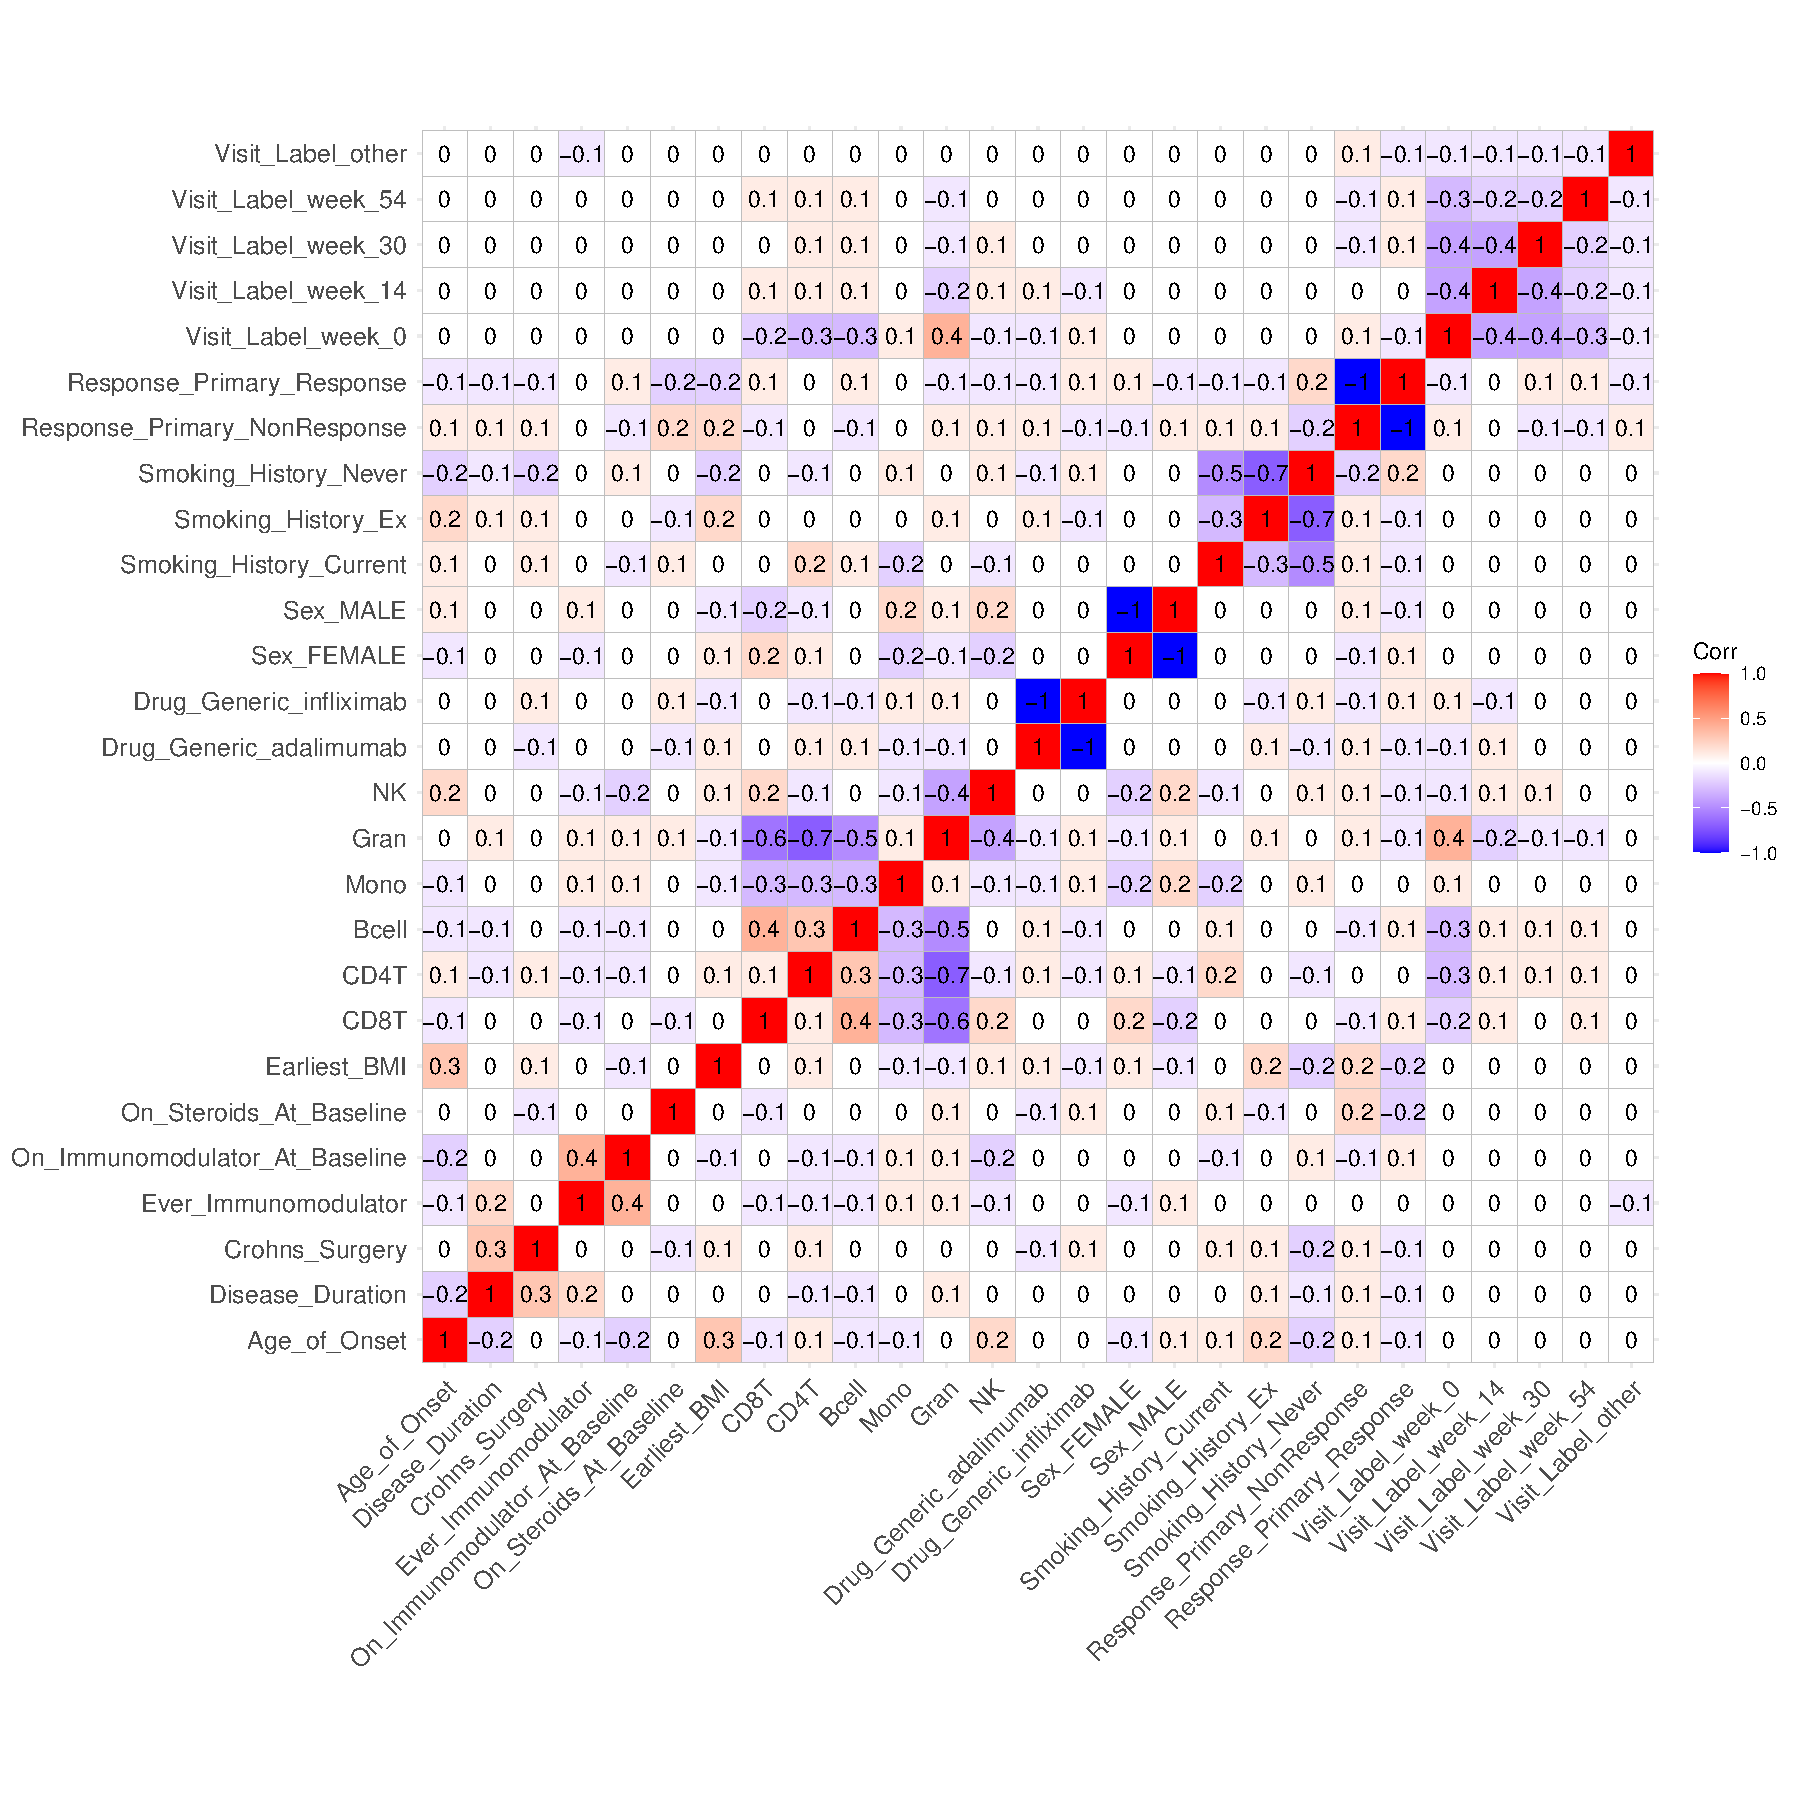
\includegraphics[width=1.0\textwidth,page=1]{mainmatter/figures/chapter_04/process_pheno.pheno_filtered_dge.ggcorrplot.pdf}
    \caption{}
    \label{fig:multipants_pheno_corrplot}
\end{figure}

A variance components analysis was conducted to identify variables that explain large fractions of variation in expression
using \software{variancePartition}\autocite{hoffman2016VariancePartitionInterpretingDrivers}, which fits a mixed regression model.
Variables in \autoref{fig:multipants_pheno_corrplot} were included as predictors.
Additional categorical variables were included for patient, \gls{RNAseq} plate, and library prep protocol version.
An additional continuous variable consisting of random numbers drawn from the standard normal distribution was also included as a null.
Granulocyte proportion estimates were dropped to relieve multicollinearity.
\todo{the var explained by Gran will be redistributed among highly cor vars anyways}
Categorical variables were coded as random effects, and continuous variables as fixed effects.
Surprisingly, \textcite{hoffman2016VariancePartitionInterpretingDrivers} showed that variance proportion estimates are unbiased even when coding categorical variables with as few as two categories as random, 
as long as all model parameters are estimated jointly using \gls{ML} rather than \gls{REML}\footnote{
    \gls{REML} treats random effects as nuisance parameters and estimates fixed effects after first integrating out random effects).
}.
This approach also avoids over-estimates of variance proportions that occur if categorical variables with many levels are treated as fixed.

\1 Variables were ranked by median variance proportion across all genes (\autoref{fig:mul}).
The variables that explained the most variance included patient, cell proportions and \gls{RNAseq} plate.
Variables that did not explain more variation on average than the null could still have high maximum values, 
indicating their importance for specific genes only, such as genes with sex-specific expression.
    \2 choice: penalty is 1 df, so include some of these low median, high max variables as covariates.
    \2 so basically select all, except Gran, and ever immunomod

\1 If covariates are also associated with the predictor X, issues can arise depending on their causal role.
In general,
conditioning on a confounder (X \textleftarrow Z \textrightarrow Y) reduces bias,
conditioning on a collider (X \textrightarrow Z \textleftarrow Y) induces bias,
and conditioning on a mediator (X \textrightarrow Z \textrightarrow Y) changes the effect estimated by removing the indirect effect mediated by Z.
    \2 Do the selected covariates have potential roles as confounders, colliders or mediators?
    \2 cell counts are potential ... confounders/mediators ... depends ...
    \todo{don't know if it matters if there are colliders among covariates, since we can't estimate any causal effects in DGE due to lack of a control group}

\todo{because this is non-randomised, baseline differences do matter}
% - pull in baseline from kennedy2019PredictorsAntiTNFTreatment
% Univariable analyses showed the strongest associations
% with primary non-response to infliximab and
% adalimumab were with week 14 drug and anti-drug
% antibody concentrations (table 3; appendix p 17). Primary
% non-response to infliximab was also associated with
% older age at first dose, smoking at baseline, non-use of an
% immunomodulator at baseline, lower baseline albumin
% concentrations, and higher baseline white cell count.
% Primary non-response to adalimumab was associated
% with a higher body-mass index at baseline.

% Sex
% Age
% BMI
% Age of Onset
% Crohn’s Surgery
% Ever Immunomodulator
% Current Smoker
% Proportions of the 6 cell types: CD4+ T cells, CD8+ T cells, B cells, NK cells, monocytes, and granulocytes

\begin{figure}
    \centering
    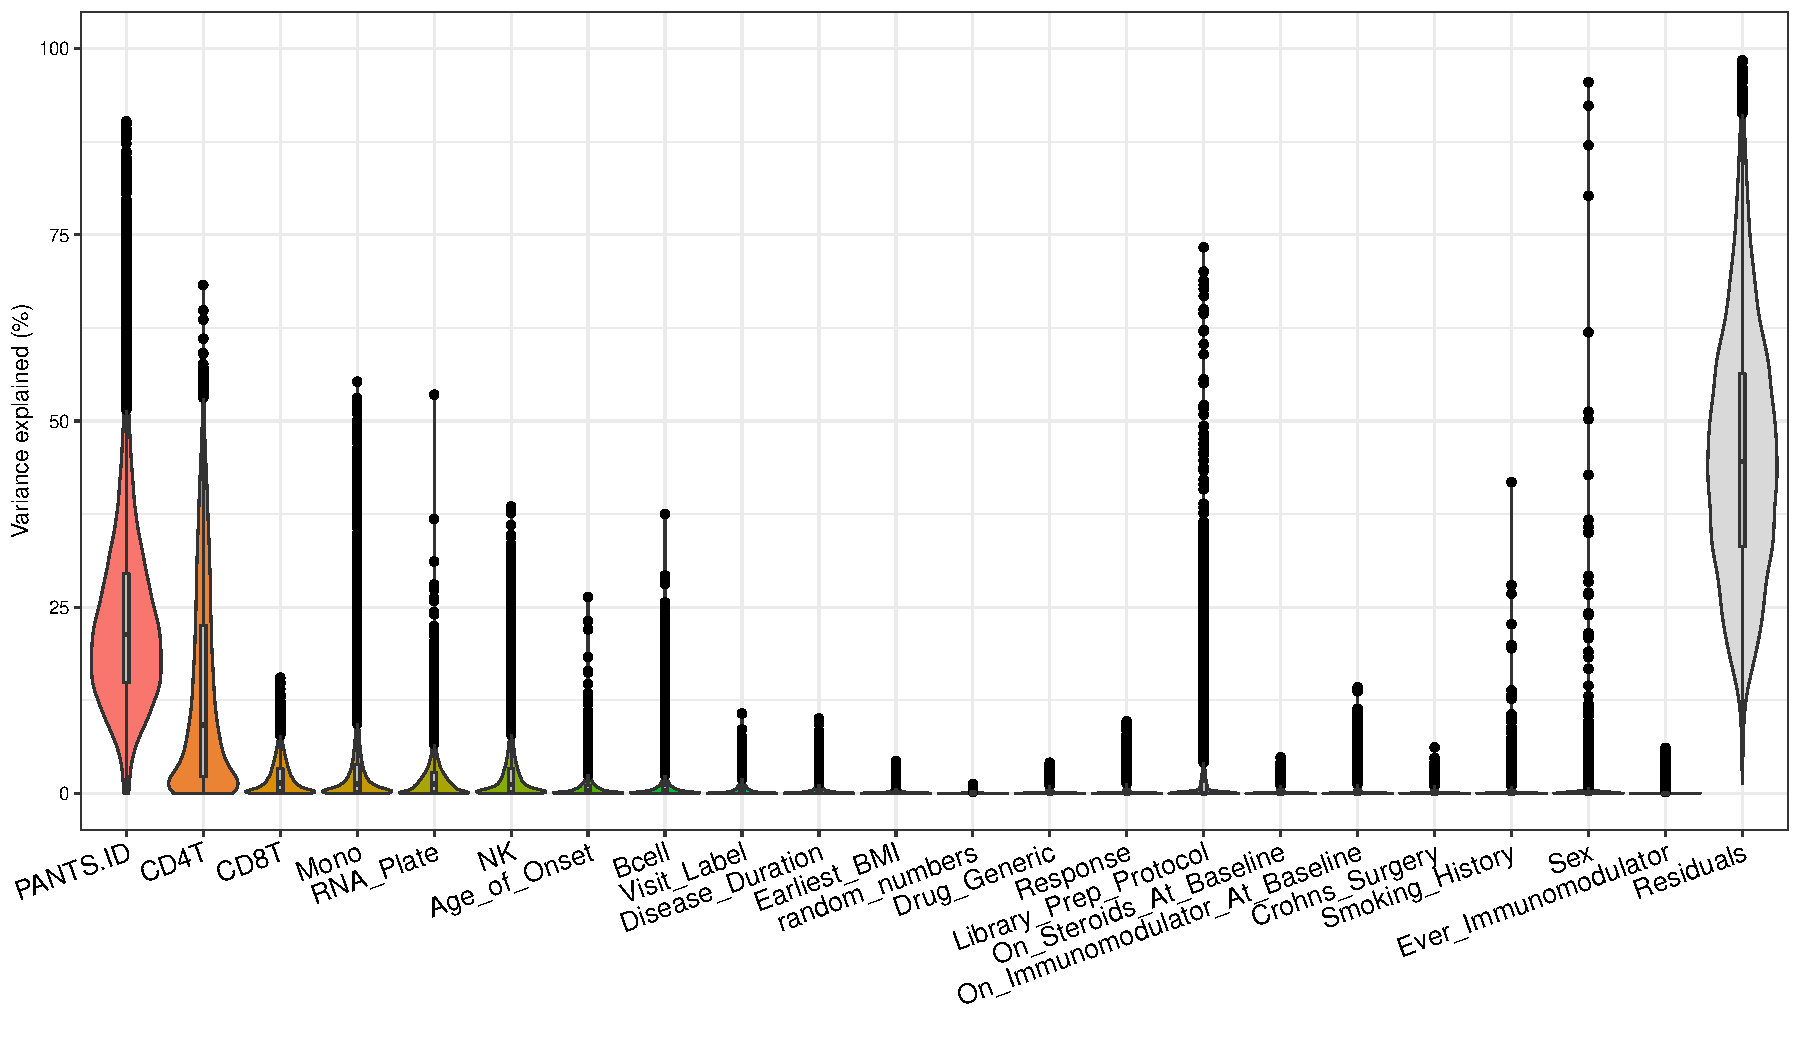
\includegraphics[width=1.0\textwidth,page=1]{mainmatter/figures/chapter_04/dream.plotVarPart.pdf}
    \caption{}
    \label{fig:multipants_varPart}
\end{figure}

\subsubsection{Contrasts model}

\software{dream} hoffman2018DreamPowerfulDifferential

8 groups equiv to 3 way interactions
12 contrasts
% dream.plotContrasts.pdf

But for dream, 
REML is TRUE, so use fixed for small numbers of levels
also, need fixedeffects for tested covariates

Dream uses lmerTest approximation Satterthwaite df \url{https://link.springer.com/article/10.3758/s13428-016-0809-y} and REML
combo controls type 1 error for n>144 in lmerTest simulations

journals need p values
% However, in the lme4 package in R the standards for evaluating significance of
% fixed effects in these models (i.e., obtaining p-values) are somewhat vague.
% There are good reasons for this, but as researchers who are using these models
% are required in many cases to report p-values, some method for evaluating the
% significance of the model output is needed.
%
% The primary motivation for this omission is that in linear mixed models it is
% not at all obvious what the appropriate denominator degrees of freedom to use
% are, except perhaps for some simple designs and nicely balanced data.

\subsubsection{Spline model}

simple time x responder interaction over time
    assumes linear change

treat time as categorical visits (like baseline/w14 analysis above), then f test all interactions
    not clean defintion of visits
    there are many intermediate visits that are not main 4

over all timepoints, are there diff trajectories for R and NR?
3 interaction terms
Internal Knots set at w14 and w30, since drug admin here, so slope should be allowed to change until next admin
TODO check What is a basis i.e. what is in the design matrix?
cubic or linear between knots?
Not sure if time is ok as continuous. Knots are approximate

\subsection{GSE}

camera is dev to use mod t, but in practice ranks are comparable between t and z.std, even though dream says otherwise
% https://bioconductor.org/packages/release/bioc/vignettes/variancePartition/inst/doc/dream.html#dream-analysis

\subsection{pred}

Sparse partial least squares regression for simultaneous dimension reduction and variable selection
% https://www.ncbi.nlm.nih.gov/pmc/articles/PMC2810828/

 Sparse Partial Least Squares Classification for High Dimensional Data 
% https://pubmed.ncbi.nlm.nih.gov/20361856/

\subsection{Genotype data preprocessing}

% sazonovs2019HLADQA105Carriage
% DNA was extracted from pretreatment blood samples from
% 1524 individuals in the PANTS cohort and genotyping undertaken
% using the Illumina CoreExome microarray
%
% After quality
% control, 1323 individuals remained in the study, of which
% 1240 had drug and anti-drug antibody level data available
% (Supplementary Figure 2).
%
% 7,578,947 variants with an information content metric score .4 were subsequently taken forward for analysis
%
% HLA types were imputed at 2- and 4-digit resolution for the
% following loci: HLA-A, HLA-C, HLA-B, HLA-DRB1, HLA-DQA1,
% HLA-DQB1, and HLA-DPB1.
%
% sex,
% drug type (infliximab or adalimumab), immunomodulator use,
% and the first within-sample principal component were
% included as covariates (Supplementary Table 2).

\subsection{reQTL}

% gutierrez-arcelus2020AllelespecificExpressionChanges

% Alternative:
% In the ANCOVA approach, the whole focus is on whether one group has a higher mean after the treatment. It’s appropriate when the research question is not about gains, growth, or changes.

% https://www.theanalysisfactor.com/pre-post-data-repeated-measures/
ANCOVA vs repeated measures vs mixed model

% The biggest advantage of mixed models is their incredible flexibility.  They can handle clustered individuals as well as repeated measures (even in the same model).  They can handle crossed random effects, where there are repeated measures not only on an individual, but also on each stimulus.
% https://www.theanalysisfactor.com/repeated-measures-approaches/

Then work out if genetics changes trajectories for any gene i.e. DGE models with a snp as predictor
First need to eQTL scan in general with mashr and find the snps in the most reQTLish genes, since this modelling is probably expensive

\section{Results}

\subsection{DGE}

% dream.gene_expr_filtered_vobj_fit_dge_1_decideTests.csv
not much DGE R vs NR at baseline
PDIA5, IGKV1-9, KCNN3 ADA only
Top ADA genes are full of IG segments, not so for IFX
Not sure which of the baseline diffs are relevant, not sure what informs the choice of ada vs ifx
some DGE R vs NR at w14
downregulated in R: immune activation, TLR and inflammatory signalling
% dream.gene_expr_filtered_vobj_fit_dge_1.topTable_C_3RI_1RI.gene_set_enrichment.tmodCERNOtest_result_LI_ascending.csv
e.g. CD177
lots of DGE baseline -> w14
more so for R than NR
more so for IFX than ADA
consistent with Abbvie
Not much diff between drugs
TODO: Add contrasts with drugs combined?
i.e. if theres no interaction, drop it
TODO: prettify GSE

% dream.gene_expr_filtered_vobj_fit_dge_2_decideTests.csv
306 signif
Not sure how much intersect with w14 pairwise

\section{Discussion}

% kennedy2019PredictorsAntiTNFTreatment
% "In our study, higher baseline markers of
% inflammation predicted lower drug concentrations at
% week 14, suggesting that higher inflammatory load might
% contribute to faster drug elimination."

% Genetic Loci associated with C-reactive
% protein levels and risk of coronary heart disease.
%
% This was recently demonstrated by
% a GWAS of C-reactive protein (CRP) levels; that study
% found that common variants near the HNF1A gene were
% associated with variation in CRP.60

\1 can we expand the PANTS conclusions to IBD and other IMIDs?
\1 source of multiomics data 1000IBD cohort \autocite{imhann20191000IBDProjectMultiomics}

"Comparative analysis of differential gene expression tools for RNA sequencing time course data"
Surprisingly, TC tools were outperformed by the classical pairwise comparison approach on short time series (<8 time points) in terms of overall performance and robustness to noise, mostly because of high number of false positives, with the exception of ImpulseDE2.

PNR definition
    its very complex
    kennedy2019PredictorsAntiTNFTreatment says once PNR, no point in continuing
        approx of remission, which has it's own def

    Binary pheno Def not rubbish
        marks fc analysis
        And remission is rare in PNR in general

Utility of the other timepoints:
    mainly seems to be maintained

Try predict drug conc?
    % Nick’s paper shows w14 drug conc is associated with PNR and remission
    % dream.pheno_df_filtered_Drug_Level_vs_Study_Day.pdf
    % About 229/329 have w14 drug conc


\end{outline}
